\section{Forging World Model}
\label{sec:world_model}

The geometry and multi-physics fields of the forging deformation sequence evolve continuously along the deformation history. To jointly carry geometry together with temperature, von Mises stress, and damage in a low-dimensional latent state and to support continuous-time autoregressive propagation, this work constructs a forging world model in the Encoder--Latent Dynamics--Decoder architecture: the encoder $E:\mathbb{R}^{N\times 6}\to\mathbb{R}^{d}$ maps the point cloud $X_k\in\mathbb{R}^{N\times 6}$ of step $k$ to a latent state $c_k=E(X_k)\in\mathbb{R}^{d}$, serving as a compact snapshot of the workpiece (geometry and multi-physics fields) at that step; the latent dynamics model $g:\mathbb{R}^{d}\times\mathbb{R}\to\mathbb{R}^{d}$ models the continuous evolution of the latent state in an augmented space, conditioned on the die speed profile; and the decoder $\mathrm{Dec}$ reconstructs the point cloud $\hat{X}_k=\mathrm{Dec}(c_k)\in\mathbb{R}^{N\times 6}$ from the latent state. The world model thus possesses both reconstruction and prediction capabilities: the former ensures that the latent state can be faithfully restored to the geometry--multi-physics point cloud, while the latter ensures that it can be propagated autoregressively along the process parameters. The overall framework of the world model is shown in Fig.~\ref{fig:world_model}.
\begin{figure}[htbp]
\centerline{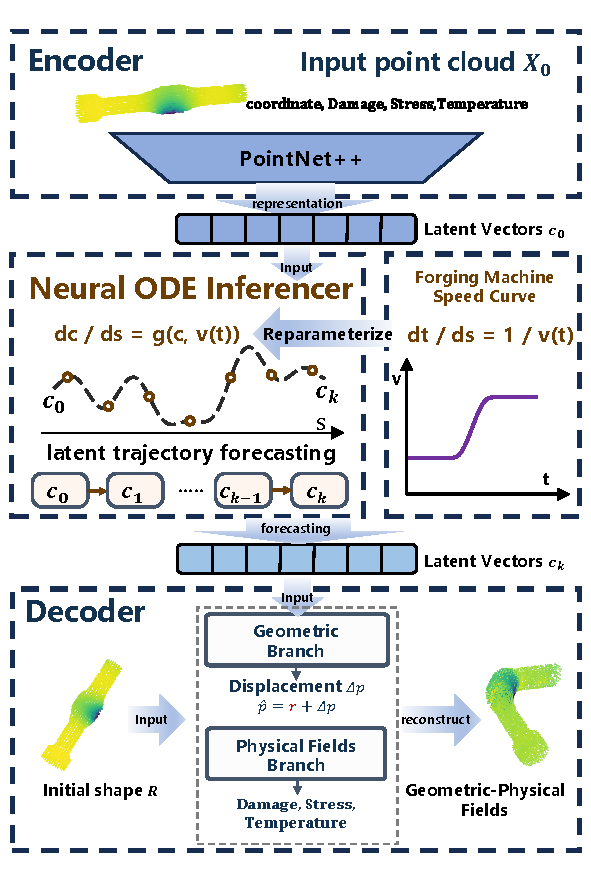
\includegraphics[width=12cm]{world_model_framework_wide.pdf}}
\caption{Overall framework of the forging world model: the encoder $E$ maps the point cloud to the latent state $c_k$, the latent dynamics model $g$ propagates the latent state along the stroke conditioned on the speed profile, and the decoder $\mathrm{Dec}$ reconstructs the geometry--multi-physics point cloud from the latent state.}
\label{fig:world_model}
\end{figure}

\subsection{Point Cloud Encoder}
Denote the point cloud of step $k$ as $X_k=\{[\,p_i;\ h_i\,]\}_{i=1}^{N}\in\mathbb{R}^{N\times 6}$, where $p_i\in\mathbb{R}^{3}$ is the absolute coordinate and $h_i=(T_i,\sigma_i,D_i)\in\mathbb{R}^{3}$ is the temperature, von Mises stress, and damage at that point, consistent with the definition in Eq.~\ref{equ:pointcloud}. The encoder builds on the hierarchical structure of PointNet++ and extracts features level by level through sampling--grouping--local aggregation.

First, farthest point sampling (FPS) selects center points deterministically by geometry. Let $S_{m-1}$ denote the set of already selected centers (initialized with $S_0$ as an arbitrary point); the $m$-th center is
\begin{equation}
p_{m}=\arg\max_{p\in\{p_i\}}\ \min_{p'\in S_{m-1}}\big\|p-p'\big\|_{2},\qquad S_{m}=S_{m-1}\cup\{p_{m}\},
\end{equation}
i.e., the point farthest from the already selected set is chosen, where $p_i$ is the coordinate of point $i$ and $S_m$ is the set of the first $m$ selected centers. This sampling is insensitive to the input order of the points. For any center point $p_i$, a ball query with radius $\delta$ obtains its local neighborhood
\begin{equation}
\Omega_i=\{\,j:\ \|p_j-p_i\|_{2}\le \delta\,\},
\end{equation}
A shared MLP is applied to each point in the neighborhood, followed by channel-wise max pooling, to obtain the local feature of the center point
\begin{equation}
f_i=\max_{j\in\Omega_i}\ \mathrm{MLP}\big([\,h_j;\ p_j-p_i\,]\big),
\end{equation}
where $f_i\in\mathbb{R}^{d_1}$ is the local feature of center $i$ ($d_1$ is the first-level feature dimension), $p_j-p_i\in\mathbb{R}^{3}$ is the coordinate of neighbor $j$ relative to the center, and $h_j\in\mathbb{R}^{3}$ is the physical-field feature of point $j$ (first layer). Repeating the above sampling--grouping--aggregation for $n_{\text{SA}}$ levels expands the receptive field from local to global.

Finally, global max pooling is applied to the last-level features followed by an MLP mapping, yielding the low-dimensional latent state that carries the state of the entire workpiece:
\begin{equation}
c_k=\mathrm{MLP}\Big(\max_{i} f_i^{(n_{\text{SA}})}\Big)\in\mathbb{R}^{d} .
\end{equation}
where $f_i^{(n_{\text{SA}})}$ is the center-point feature output by the $n_{\text{SA}}$-th (last) level, $\max_i$ denotes channel-wise max over all center points, and $d$ is the latent-state dimension. Since sampling and grouping depend only on geometric distances and the neighborhood information is aggregated by symmetric max pooling, the encoder is permutation-invariant with respect to the input order of points, i.e., $E(\Pi(X_k))=E(X_k)$ for any permutation $\Pi$.

\subsection{Latent Dynamics Model}
The conditional input of the latent dynamics model is the die speed profile $v_y(t)$, which can be any continuous curve; the curves in the training data are generated by low-dimensional parameterized sampling, covering constant-speed, fast-then-slow, slow-then-fast, and other shapes. The speed value is normalized and fed into the vector field to be learned together with the latent state.

On this basis, the latent dynamics model describes the continuous evolution of the latent state in the augmented ``physical-time--latent-state'' space: taking the stroke $s$ (the downward displacement of the press) as the integration variable, from $ds=v_y(t)\,dt$ we have
\begin{equation}
\frac{dc}{ds}=g\big(c,\,v_y(t)\big),\qquad \frac{dt}{ds}=\frac{1}{v_y(t)} ,
\end{equation}
where $c\in\mathbb{R}^{d}$ is the latent state, $g:\mathbb{R}^{d}\times\mathbb{R}\to\mathbb{R}^{d}$ is the vector field to be learned (parameterized by an MLP), and $t$ and $s$ are the physical time and stroke, respectively. The latent dynamics model thus integrates step by step along the stroke $s$, while the speed profile is given with the physical time $t$ as the independent variable; the two are converted through $ds=v_y(t)\,dt$ (equivalently $dt/ds=1/v_y(t)$), and the physical time $t$ advances synchronously with the integration as an augmented state, i.e., the integration step is taken in displacement while the speed is expressed on the time axis. The speed profile is thereby embedded as a physical prior into the time-scale transformation, aligning the prediction time scale with the true process. The latent state of two adjacent steps is obtained by integrating over the interval:
\begin{equation}
c_{k+1}=c_k+\int_{s_k}^{s_{k+1}} g\big(c(s),\,v_y(t(s))\big)\,ds ,
\end{equation}
where $s_k$ and $s_{k+1}$ are the strokes corresponding to two adjacent steps, and $c(s)$ is the latent state evolving along the stroke. This differential equation is solved by the fourth-order Runge--Kutta method, with backpropagation performed via the adjoint method. Because the latent dynamics model integrates over the stroke with the speed profile given analytically, the integration step need not coincide with the training step: training uses a fine step to constrain the local dynamics, while inference uses a coarse step to cover the entire history, with both sharing the same vector field.

\subsection{Joint Geometry--Physics Decoder}
The decoder adopts a DeepONet structure and learns an operator $\mathrm{Dec}$ mapping the latent state to a displacement--physics-field map: the branch network takes the latent state $c_k$ as input, the trunk network takes the reference coordinate $r_i$ as the query point, and after tensor fusion a shared output layer jointly produces the displacement and physical fields at that point. The overall structure of the decoder is shown in Fig.~\ref{fig:decoder}. Taking the query coordinate as the trunk input enables the decoder to query arbitrary reference points and share a spatial basis across points, so that a single network characterizes the field distribution over the entire point cloud. Let the first-step geometry be $R=\{r_i\}_{i=1}^{N}$ ($r_i\in\mathbb{R}^{3}$ is the coordinate of the $i$-th reference point), i.e., the first-step point cloud of this sample (denoted $X_0$), the initial geometry of the workpiece; it is a known input in both training and inference and varies sample by sample with the initial condition. The point-wise action of the decoder on each reference point is
\begin{equation}
\begin{aligned}
\hat{y}_i&=\big(\hat{T}_i,\ \hat{\sigma}_i,\ \hat{D}_i\big),\\
\big[\,\Delta p_i;\ \hat{y}_i\,\big]&=W\big(f_{b}(c_k)\otimes f_{t}(r_i)\big)+b,
\end{aligned}
\end{equation}
where $f_{b}:\mathbb{R}^{d}\to\mathbb{R}^{P\times C}$ and $f_{t}:\mathbb{R}^{3}\to\mathbb{R}^{P}$ are the branch and trunk networks, $P$ is the number of spatial bases, and $C=6$ is the number of output channels (3 displacement dimensions and 3 physical fields); $W\in\mathbb{R}^{C\times(PC)}$ and $b\in\mathbb{R}^{C}$ are the weight and bias of the output layer; $\Delta p_i\in\mathbb{R}^{3}$ is the displacement prediction of reference point $i$, and $\hat{T}_i$, $\hat{\sigma}_i$, $\hat{D}_i$ are the predicted temperature, von Mises stress, and damage, respectively. Let $\mathrm{Dec}(c_k)$ denote the complete point cloud generated from $c_k$; its point-wise action on any reference point $r_i$ is exactly the above equation. The displacement and physical fields are coupled from the same latent state through a shared output layer, constraining each other physically.

\begin{figure}[htbp]
\centerline{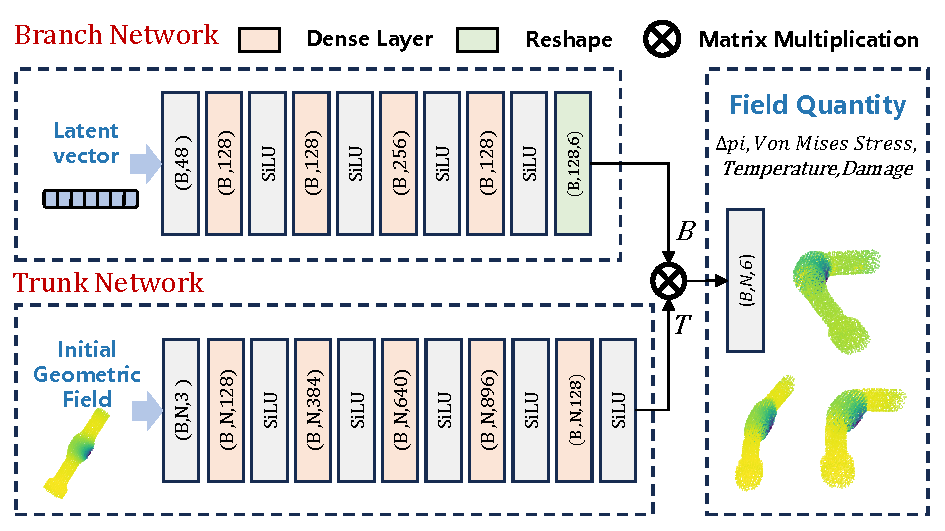
\includegraphics[width=12cm]{decoder-wide.pdf}}
\caption{Schematic of the decoder architecture.}
\label{fig:decoder}
\end{figure}

\textbf{Geometry.} With the first-step geometry $R$ as a hard baseline, the network predicts only the relative displacement:
\begin{equation}
\hat{p}_i=r_i+\Delta p_i .
\end{equation}
When there is no deformation, $\Delta p_i\approx0$, i.e., $\hat{p}_i\approx r_i$; this residual form converts ``reconstructing the geometry'' into ``learning the displacement'', which both reduces the learning difficulty and ensures that the initial shape is exactly restored.

\textbf{Physical fields.} The three physical fields are regressed using the same reference coordinate $r_i$ as the query point. Since the query coordinate always takes the reference point $r_i$ in the first-step geometry $R$ (the index is the material-point identity) during both training and inference, the input distribution of the two stages remains consistent, avoiding distribution shift caused by geometric evolution. Accordingly, geometry and physical fields are jointly output point by point from the same latent state to reconstruct the point cloud:
\begin{equation}
\hat{X}_k=\big\{\,(\hat{p}_i,\ \hat{y}_i)\,\big\}_{i=1}^{N},
\end{equation}
yielding $\hat{X}_k\in\mathbb{R}^{N\times 6}$, which jointly reconstructs the shape and multi-physics fields from the same latent state and reinforces the physical consistency between geometry and fields.

\subsection{Training Objective}
The world model is trained in two stages. In the first stage, the encoder and decoder are trained with only the reconstruction loss, so that the latent state can be reconstructed into the geometry--multi-physics point cloud. In the second stage, the latent dynamics model is trained with a latent-space prediction loss and a multi-step rollout loss to optimize its vector field, so that the latent state can be propagated autoregressively along the die speed profile.

The reconstruction loss of the first stage is the point-wise error of the point cloud reconstructed by the decoder from the true latent state, summed over all steps and averaged over the batch ($\mathbb{E}[\cdot]$ denotes the expectation over the batch):
\begin{equation}
\mathcal{L}_{\text{recon}}=\mathbb{E}\Big[\sum_{k}\big\|\mathrm{Dec}(c_k)-X_k\big\|^{2}\Big] .
\end{equation}

The latent-space prediction loss of the second stage is the mean squared error between the predicted latent state and the true encoding, where $\hat{c}_{k+1}$ is the next latent state predicted by the latent dynamics model, $c_{k+1}=E(X_{k+1})$ is the corresponding true encoding, and $\mathrm{sg}(\cdot)$ is the stop-gradient operator (cutting off gradient backpropagation to the encoder):
\begin{equation}
\mathcal{L}_{\text{pred}}=\mathbb{E}\Big[\big\|\hat{c}_{k+1}-\mathrm{sg}(c_{k+1})\big\|^{2}\Big] .
\end{equation}

The multi-step rollout loss enhances long-horizon prediction stability and is combined with the prediction loss via weight $\beta_M$: starting from step $k$, an $M$-step autoregressive rollout is performed, where each step advances from the latent state predicted at the previous step rather than using the true encoding, and the loss is computed between the predicted latent state at each step on the rollout path and the true encoding of that step:
\begin{equation}
\mathcal{L}_{\text{rollout}}=\mathbb{E}\Big[\sum_{k}\sum_{j=1}^{M}\big\|\hat{c}_{k}^{(j)}-\mathrm{sg}(c_{k+j})\big\|^{2}\Big],
\end{equation}
where the autoregressive rollout is
\begin{equation}
\begin{aligned}
\hat{c}_{k}^{(0)} &= \mathrm{sg}(c_k), \\
\hat{c}_{k}^{(j+1)} &= \hat{c}_{k}^{(j)}+\int_{s_{k+j}}^{s_{k+j+1}} g\big(\hat{c}_{k}^{(j)},\,v_y(t(s))\big)\,ds ,
\end{aligned}
\end{equation}
$\hat{c}_{k}^{(j)}$ is the predicted latent state after rolling out $j$ steps from step $k$, and $c_{k+j}=E(X_{k+j})$ is the true encoding of the corresponding step; the prediction at each step on the rollout path is directly supervised by the true encoding of that step.
